\clearpage
\section{Dokonalá konkurence (charakteristiky, tržní rovnováha a její efektivnost, přebytek
spotřebitele a přebytek výrobce, typy nerovnováhy).}

\subsection{Charakteristiky}
\begin{enumerate}
    \item \textbf{Velké množství prodávajících a nakupujících} (Velké množství nakupujících 
    umožňuje, aby firmy nebyly v područí jediného odběratele.)
    \item \textbf{Dokonalá informovanost kupujících} (splněno při burzách. V případě trhů 
    územně rozptýlených, jako jsou např. restaurační služby, hotely, cukrárny atp. nemívají
    kupující k dispozici všechny informace )
    \item \textbf{Homogenní produkt} (spotřebitel se rozhoduje o koupi výrobku výlučně podle
    ceny, nebere v úvahu jiná hlediska, např. kvalitu výrobku či pověst firmy. Tuto podmínku
    splňuje jen málo výrobků a služeb)
    \item \textbf{Volný vstup na trh} (a výstup z tohoto trhu) - spojeno s překážkami vstupu do odvětví.
    \begin{itemize}
        \item Žádné překážky vstupu (prodej textilu, webdesign, vedení účetnictví)
        \item Velké překážky vstupu (výroba elektřiny a její distribuce, či proniknutí
        na trh s operačními systémy pro PC) Typické překážky:
        \begin{itemize}
            \item vysoké fixní náklady
            \item kontrola zdrojů, nezbytných pro výrobu, jedinou firmou
            \item právní restrikce v podobě patentů, ochranných práv autorů
            \item udělení výsadního práva pro činnost firmy státem
        \end{itemize}
    \end{itemize}
    \item \textbf{Nulové náklady na změnu dodavatele} (pokud se rozhodne kupující změnit 
    dodavatele, tak jej tato změna nic nestojí žádné dodatečné náklady)
\end{enumerate}

\subsection{Tržní rovnováha}
Nastává, když se mezní užitek statku rovná mezním nákladům na jeho výrobu. 
Tržní rovnováha je pro ekonomickou realitu jev výjimečný.\\
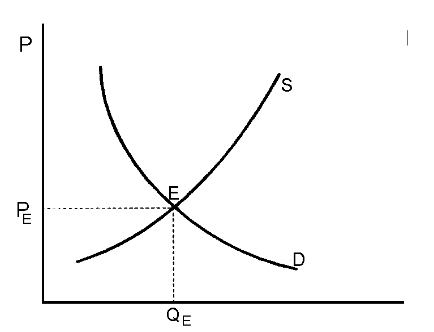
\includegraphics{images/11_trzni_rovnovaha.png}\\
\textbf{Efektivnost} spočívá v porovnání mezního užitku a mezních nákladů. Z toho vyplývá,
že společensky efektivní tržní produkcí je taková produkce statku, jejíž mezní užitek se rovná mezním
nákladům. Jinými slovy tržní rovnováha nastává v průsečíku křivky poptávky a křivky nabídky, neboť
tam se poptávané množství právě rovná nabízenému množství.

\subsection{Přebytek spotřebitele}
Je kumulativní rozdíl mezi částkou, kterou kupující byli ochotni zaplatit
za statek, a jeho skutečnou cenou na trhu.

\subsection{Přebytek výrobce}
Je rozdíl mezi celkovými příjmy firmy a součtem mezních nákladů.

\subsection{Typy nerovnováhy}
\begin{enumerate}
    \item \textbf{Tržní nedostatek} – poptávané množství převyšuje nabízené množství.
    Nedostatek vzniká, když je cena nižší než rovnovážná cena.
    \item \textbf{Tržní přebytek} – nabízené množství převyšuje poptávané množství. 
    Přebytek vzniká, když je cena vyšší než rovnovážná cena.
\end{enumerate}